\title{Developing Inference Algorithms}

{{navbar}}

\subsubsection{Developing Inference Algorithms}

Edward uses class inheritance to provide a hierarchy of inference
methods. This enables fast experimentation on top of existing
algorithms, whether it be developing new black box algorithms or
new model-specific algorithms.
For examples of algorithms developed in Edward, see the inference
\href{/tutorials/}{tutorials}.

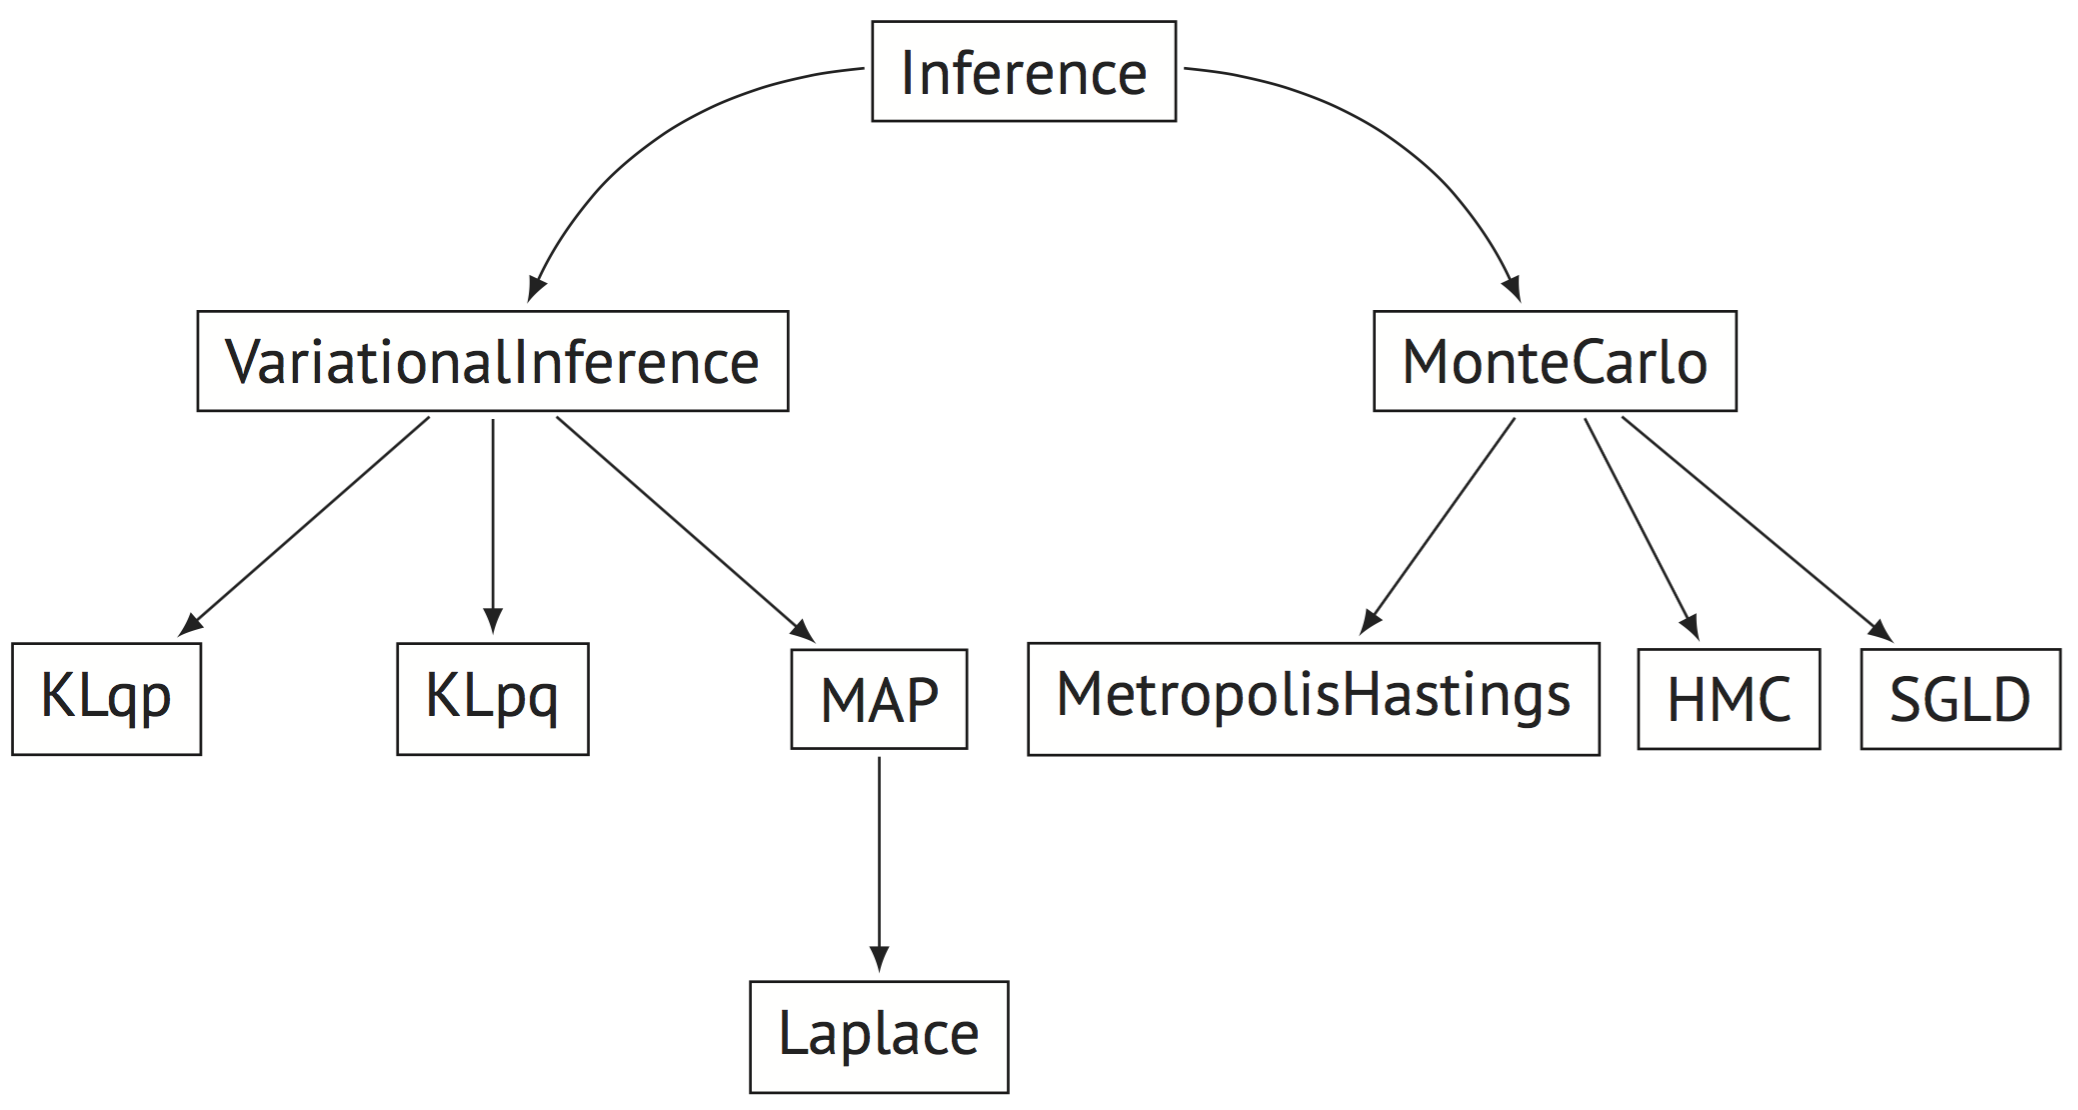
\includegraphics[width=700px]{/images/inference_structure.png}
{\small\textit{Dependency graph of several inference methods.
Nodes are classes in Edward and arrows represent class inheritance.}}

There is a base class \texttt{Inference}, from which all inference
methods are derived from. Note that \texttt{Inference} says nothing
about the class of models that an algorithm must work with. One can
build inference algorithms which are tailored to a restricted class of
models available in Edward (such as differentiable models or
conditionally conjugate models), or even tailor it to a single model.
The algorithm can raise an error if the model is outside this class.

We organize inference under two paradigms:
\texttt{VariationalInference} and \texttt{MonteCarlo} (or more plainly,
optimization and sampling). These inherit from \texttt{Inference} and each
have their own default methods.

For example, developing a new variational inference algorithm is as simple as
inheriting from \texttt{VariationalInference} and writing a
\texttt{build\_loss\_and\_gradients()} method. \texttt{VariationalInference} implements many default methods such
as \texttt{initialize()} with options for an optimizer.
For example, see the
\href{https://github.com/blei-lab/edward/blob/master/examples/iwvi.py}{importance
weighted variational inference} script.
